\begin{abstract}
With the increasing adoption of cloud resources, public and private, to support
the demands in terms of computing capacity for WLCG, the HEP community has begun
studying several benchmarking applications aimed at continuously assessing the
performance of virtual machines procured from commercial providers.
In order to characterise the behaviour of these benchmarks, in-depth
profiling activities have been carried out. In this document we outline
our experience in profiling one specific application, ATLAS Kit Validation,
in an attempt to explain an unexpected distribution of the performance samples
obtained on systems based on Intel Haswell-EP processors.
\end{abstract}


\section{Introduction}

Nowadays the majority of the experiments' workloads running on WLCG are simulation jobs, where most of the computing time is spent in number crunching, a CPU-bound activity. For this reason the adoption of fast benchmarks representative of CPU-bound workloads can be beneficial in the grid activity for monitoring and resource match-making purposes in order to  provide real-time information about the delivered performance of a virtual machine in a cloud IaaS or a job slot in a grid site.
For instance a prompt benchmarking can  act as a prediction mechanism for the execution of the LHC experiments' workloads, allowing for a fast and reliable triage of suitable resources in a much shorter time period than standard jobs.
%
A number of fast benchmarks is being studied by the HEP community. Within the HEPiX Benchmarking Working Group~\cite{HEPiX:2014:HEPiX}, two fast benchmarks are in particular under deep investigation: Dirac Benchmark 2012 (DB12)~\cite{CERN:2016:DB12} and ATLAS Kit Validation (KV)~\cite{KV}.

\section{KV Benchmark}

KV is the toolkit adopted by the ATLAS collaboration for the
validation of their software installation in grid sites. The tests include, among
others, the GEANT4~\cite{GEANT4} simulation of the ATLAS detector. 
This test has been repurposed to benchmark compute resources against CPU-bound workloads. 
The KV benchmark simulates
$n$ independent events consisting of a single muon particle propagating through
the ATLAS detector.  The CPU time needed to simulate each event is recorded and the average over the $n$ events is computed as the final benchmark result.
Attention is paid to remove  from the measurement spurious effects such as the overhead coming from the initialisation of the
software libraries and the configuration of the simulation parameters (detector
geometry, list of particles, properties of the materials). To avoid that the first event in the sequence is excluded from the final average.

The KV benchmark is single threaded as most of the LHC experiments'
software applications. In order to fully load the compute resources and reproduce
the worst case load scenario, where all the compute slots are running jobs and
CPU idle time is minimised, the benchmarking procedure is configured to run,
by default, in parallel with as many threads as the number of logical cores of
the server and the benchmark result is calculated as the arithmetic average over
the set of threads.


In the past few years the KV benchmark measurements have been performed in several commercial cloud providers and grid sites 
where experiments' job were also running. The  benchmark results have been then compared with the average CPU time spent by the VM to simulate ATLAS events, as reported by the experiment's job monitoring framework. Details about this activity and the correlation among benchmark results and job duration are reported in~\cite{bmk}.




\section{An unexpected behaviour}
Among other environments, the KV benchmark was executed on 240 Haswell-EP hypervisors providing compute
resources as VMs dedicated to the CERN Tier-0 batch system. The servers were
fitted with two 8-core Intel Xeon E5-2630v3 processors, with a total number  
of 32 threads per server with simultaneous multithreading enabled, and 64~GiB    
of DDR4 RAM in fully balanced configuration, with each memory channel populated with
the same number of DIMMs of equal capacity. All the hypervisors were configured 
to host 2 VMs providing 16 virtual processing units each, with pairs of VMs 
confined to separate NUMA domains. KV was executed with 16 parallel processes 
on each VM, resulting in the full utilisation of the hardware threads provided
by the machine, and the final aggregated result was obtained as the average over 
the 16 simulation times. The samples collected from the VMs under test resulted in a dual-mode guassian distribution, with a 2\% difference between the 
mean of the two modes as shown in Figure~\ref{dual-mode-gaussian}.


\begin{figure}[ht]
\begin{center}
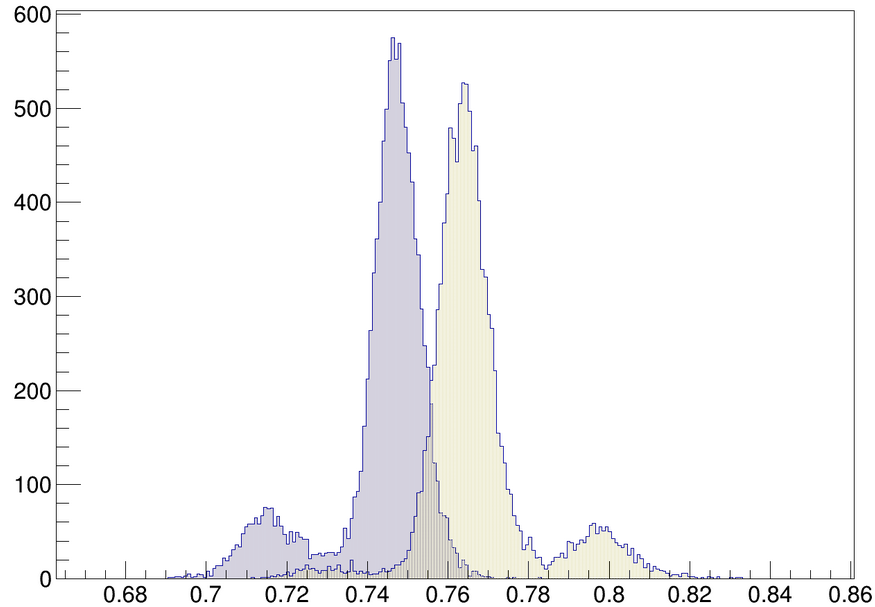
\includegraphics[width=0.5\textwidth]{images/dual-mode-gaussian.png}
\end{center}
\caption{\label{dual-mode-gaussian} Distribution of the average KV execution speed [sec/evt] from VMs with 16 virtual CPUs. }
\end{figure}


